% Prezentacja - etap 3 (28.X), wersja na 7 minut. Pełna wersja: prezentacja.tex.
% Kompilacja (XeLaTeX):  tectonic prezentacja.tex   (albo ../../prezentacja/build.sh nie dotyczy etapu 3)
\documentclass[aspectratio=169,11pt]{beamer}

\usetheme[progressbar=frametitle,numbering=fraction]{metropolis}
\usepackage[polish]{babel}
\usepackage{booktabs}
\usepackage{tabularx}
\usepackage{listings}
\usepackage{xcolor}
\usepackage{amssymb}
\usepackage{tikz}
\usetikzlibrary{arrows.meta,positioning}

\graphicspath{{../diagramy/}{img/}}
\newcolumntype{L}{>{\raggedright\arraybackslash}X}

\definecolor{ok}{HTML}{11804B}
\definecolor{bad}{HTML}{C0392B}
\definecolor{warn}{HTML}{A15C00}
\definecolor{acc}{HTML}{1F5EFF}
\newcommand{\good}[1]{\textcolor{ok}{#1}}
\newcommand{\bad}[1]{\textcolor{bad}{#1}}

\lstset{
  basicstyle=\ttfamily\footnotesize,
  keywordstyle=\color{acc}\bfseries,
  commentstyle=\color{gray},
  language=Python,
  columns=fullflexible,
  keepspaces=true,
  frame=none,
  backgroundcolor=\color{black!4},
  xleftmargin=4pt, framexleftmargin=4pt,
  extendedchars=true,
  literate={ą}{{\k{a}}}1 {ę}{{\k{e}}}1 {ó}{{\'o}}1 {ś}{{\'s}}1 {ł}{{\l}}1 {ż}{{\.z}}1 {ź}{{\'z}}1 {ć}{{\'c}}1 {ń}{{\'n}}1,
}

% pełnoekranowy diagram
\newcommand{\fullimage}[2][0.98]{%
  \begin{frame}[plain]
    \begin{tikzpicture}[remember picture, overlay]
      \node at (current page.center) {\includegraphics[width=0.99\paperwidth,height=#1\paperheight,keepaspectratio]{#2}};
    \end{tikzpicture}
  \end{frame}}

\title{System zapisów na zajęcia -- USOSv2}
\subtitle{Etap 3: projekt wstępny systemu (wersja 7 min)}
\author{Kamil Kręcigłowa \and Bartosz Królik \and Krzysztof Krówka}
\institute{Inżynieria Oprogramowania, zima 2026/2027}
\date{28 października 2026}

\begin{document}


\maketitle

% 1 ------------------------------------------------------------------ 0:45
\begin{frame}{Trzy decyzje etapu 3}
  \begin{columns}[T]
    \begin{column}{0.32\textwidth}
      \textbf{1. Tury per kierunek}\\[2pt]
      \small 20\,000 studentów nie zapisuje się naraz -- kolejny kierunek co 30 min, w szczycie ok.\ 1000 osób.
    \end{column}
    \begin{column}{0.32\textwidth}
      \textbf{2. Reguły w kodzie}\\[2pt]
      \small kolizje, wymagania, tury -- czyste funkcje w Pythonie. Baza: tylko ograniczenia i blokady (siatka bezpieczeństwa).
    \end{column}
    \begin{column}{0.32\textwidth}
      \textbf{3. Projekt = działający kod}\\[2pt]
      \small diagramy klas i sekwencji opisują implementację; 35 testów, test obciążeniowy 20\,000 kont.
    \end{column}
  \end{columns}
  \vspace{10pt}
  \footnotesize Pełna dokumentacja: \texttt{etap3/README.md} -- wszystkie przypadki użycia (UC0--UC27), 7 sekwencji, 3 diagramy klas z opisem metod, ER, uprawnienia, kody błędów.
\end{frame}

% 2 ------------------------------------------------------------------ 1:45
\begin{frame}{Architektura i stos technologiczny}
  \begin{columns}[c]
    \begin{column}{0.58\textwidth}
      \centering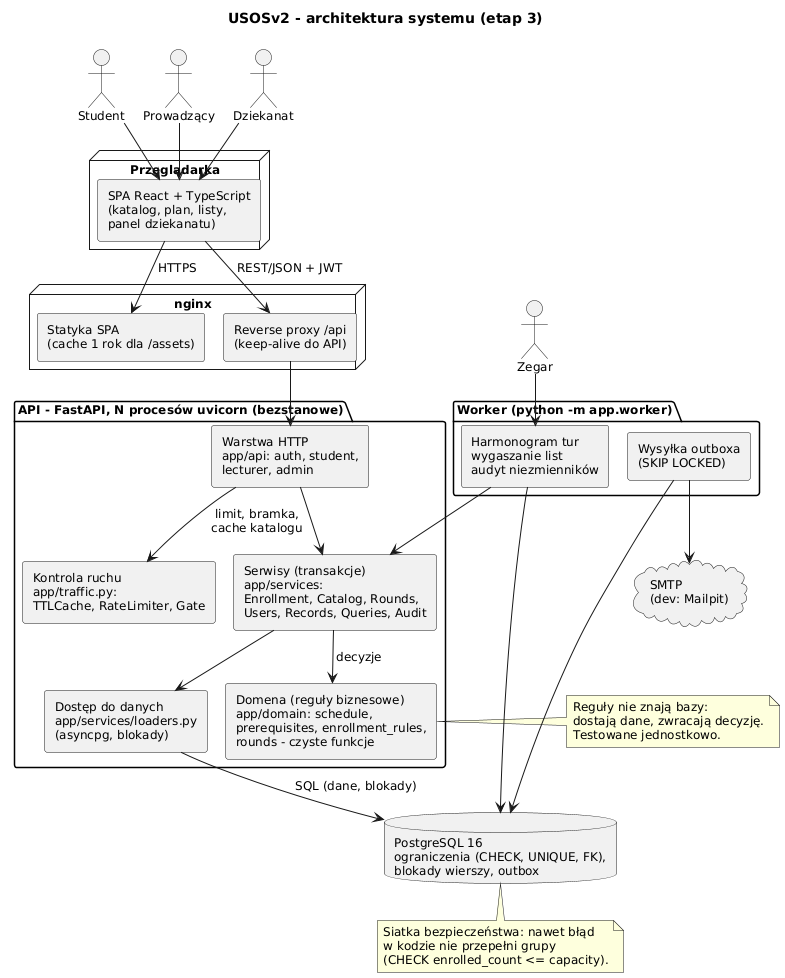
\includegraphics[height=0.82\textheight]{architektura.png}
    \end{column}
    \begin{column}{0.4\textwidth}
      \scriptsize
      \begin{tabular}{@{}ll@{}}
        \toprule
        SPA & React 19 + TypeScript \\
        WWW & nginx (statyka, proxy) \\
        API & Python 3.12, FastAPI \\
        dane & SQLAlchemy 2, asyncpg \\
        baza & PostgreSQL 16 \\
        w tle & worker (asyncio) \\
        auth & JWT 12\,h, bcrypt \\
        testy & pytest, k6 \\
        \bottomrule
      \end{tabular}\\[6pt]
      \footnotesize
      \textbf{Zasada:} warstwa HTTP $\rightarrow$ serwis (= transakcja) $\rightarrow$ domena decyduje, \texttt{loaders} czytają i zapisują.\\[3pt]
      API bezstanowe -- skalowanie kolejnymi instancjami.
    \end{column}
  \end{columns}
\end{frame}

% 3 ------------------------------------------------------------------ 2:30
\fullimage{przypadki_uzycia_student.png}

% 4 ------------------------------------------------------------------ 3:30
\fullimage[0.92]{sekwencja_zapis_skrot.png}

% 5 ------------------------------------------------------------------ 4:15
\fullimage[0.92]{sekwencja_awans_skrot.png}

% 6 ------------------------------------------------------------------ 5:00
\begin{frame}{Projekt klas: reguły w domenie}
  \centering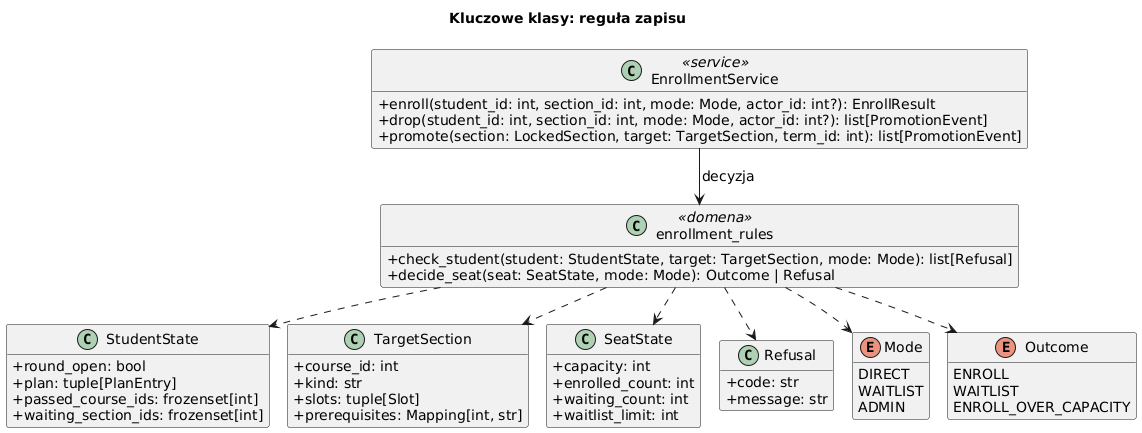
\includegraphics[width=\textwidth,height=0.7\textheight,keepaspectratio]{klasy_skrot.png}\\[2pt]
  \footnotesize Dwa kroki = dwie blokady: \texttt{check\_student} (plan studenta), potem \texttt{decide\_seat} (miejsce w grupie).
  Pełne diagramy klas (domena, serwisy, infrastruktura) z opisem metod -- zapas i \texttt{README.md} §7.
\end{frame}

% 7 ------------------------------------------------------------------ 5:35
\fullimage{er.pdf}

% 8 ------------------------------------------------------------------ 6:40
\begin{frame}{Duży ruch: zmierzone, nie założone}
  \footnotesize
  k6: każdy student przegląda katalog i zapisuje się na 6 przedmiotów (wykład + laboratorium).\\[4pt]
  \begin{tabularx}{\textwidth}{@{}L>{\raggedleft}p{1.7cm}>{\raggedleft}p{1.9cm}>{\raggedleft\arraybackslash}p{3.2cm}@{}}
    \toprule
    \textbf{Scenariusz} & \textbf{p95 zapisu} & \textbf{sesja} & \textbf{ponowienia / spójność} \\
    \midrule
    1 kierunek (1000 osób) -- pierwsza wersja & 2,5\,s & 2\,min & \bad{22\,873}, OK \\
    1 kierunek (1000 osób) -- po poprawkach & \good{1,9\,s} & \good{17\,s} & \good{0}, OK \\
    3 kierunki naraz (3000 osób) & 2,1\,s & 49\,s & 0,5\,\% nieudanych, \good{0 przepełnień} \\
    \bottomrule
  \end{tabularx}\\[6pt]
  \begin{itemize}
    \item \textbf{ograniczamy}: tury per kierunek; \textbf{obsługujemy}: krótkie blokady, bramka (503 + Retry-After), cache, bez ORM w gorącej ścieżce
    \item pomiar znalazł błąd: limit liczył ponowienia $\Rightarrow$ kaskada 429
    \item przeciążenie: wolniej, ale spójnie $\Rightarrow$ tury per kierunek są konieczne
  \end{itemize}
\end{frame}

% 9 ------------------------------------------------------------------ 7:00
\begin{frame}[standout]
  Dziękujemy -- pytania?\\[8pt]
  \normalsize dalej: slajdy zapasowe (pozostałe diagramy)
\end{frame}

% --------------------------------------------------------------------------
% Zapas: pokazywane tylko przy pytaniach.
\appendix
\section{Slajdy zapasowe}

\fullimage{przypadki_uzycia_administracja.png}
\fullimage{sekwencja_zapis.png}
\fullimage{sekwencja_wypis_awans.png}
\fullimage{sekwencja_tura.png}
\fullimage{sekwencja_dziekanat.png}
\fullimage{sekwencja_harmonogram.png}
\fullimage{sekwencja_wymagania_import.png}
\fullimage{sekwencja_logowanie.png}
\fullimage{klasy_domena.png}
\fullimage{klasy_serwisy.png}
\fullimage{klasy_infrastruktura.png}

\begin{frame}{Uprawnienia ról i obsługa błędów}
  \begin{columns}[T]
    \begin{column}{0.5\textwidth}
      \footnotesize
      \begin{tabular}{@{}lccc@{}}
        \toprule
        & \textbf{Stud.} & \textbf{Prow.} & \textbf{Dziek.} \\
        \midrule
        katalog & \good{$\checkmark$} & \good{$\checkmark$} & \good{$\checkmark$} \\
        własne zapisy, plan, listy & \good{$\checkmark$} & -- & -- \\
        listy studentów grupy & -- & swoje & \good{$\checkmark$} \\
        katalog, harmonogram, limity & -- & -- & \good{$\checkmark$} \\
        decyzje o zapisach & -- & -- & \good{$\checkmark$} \\
        tury, konta, oceny, audyt & -- & -- & \good{$\checkmark$} \\
        \bottomrule
      \end{tabular}
    \end{column}
    \begin{column}{0.46\textwidth}
      \footnotesize
      \texttt{\{code, message, details\}}
      \begin{itemize}
        \item 409 -- odmowa z powodem
        \item 429 / 503 + Retry-After -- SPA ponawia
        \item 401 / 403 / 404 / 422
        \item deadlock, \texttt{NOWAIT} -- ponawiane w transakcji
      \end{itemize}
    \end{column}
  \end{columns}
\end{frame}

\begin{frame}{Implementacja: ekrany}
  \begin{columns}[T]
    \begin{column}{0.5\textwidth}
      \centering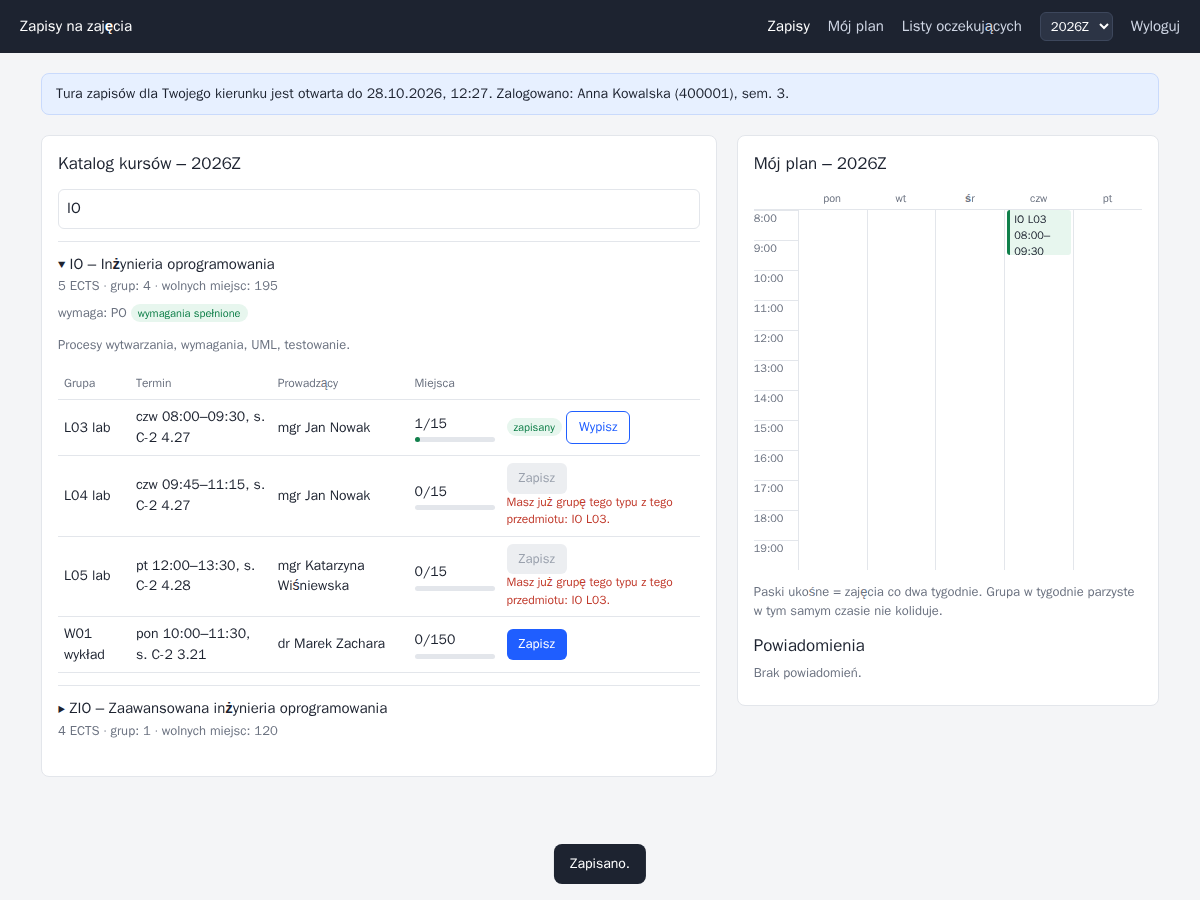
\includegraphics[width=\textwidth]{student_zapisy.png}
    \end{column}
    \begin{column}{0.5\textwidth}
      \centering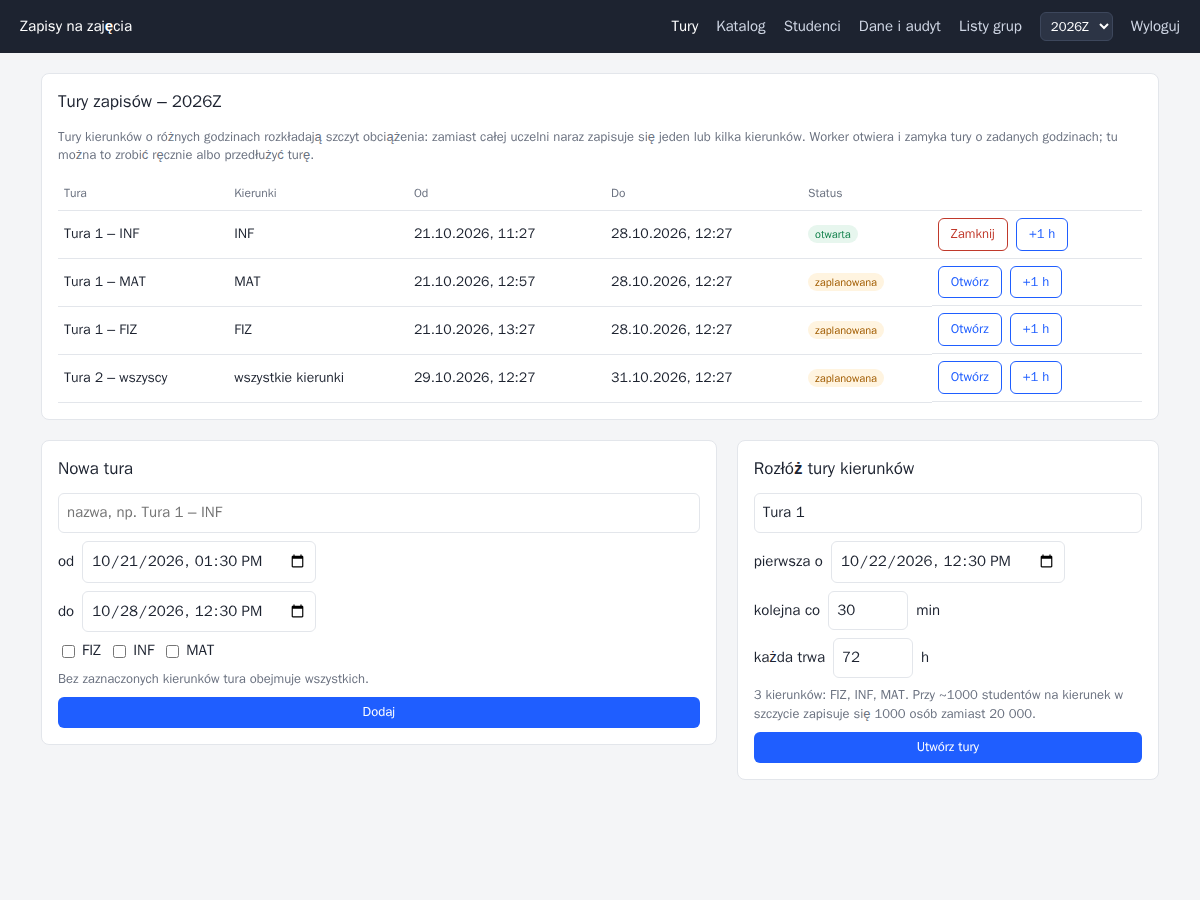
\includegraphics[width=\textwidth]{dziekanat_tury.png}
    \end{column}
  \end{columns}
\end{frame}

\end{document}
